\chapter{Abstraction}\label{C:abstraction}

% potential examples of abstraction?
% recipies
% programming?
% ???

What do I mean by abstraction?
Capturing the 'essence' of the problem. Without unimportant details.

Related. Representation learning.

What is it?
- Single elements are more complex, but tailored to specific tasks?!
- An idealisation, that ignores unimportant details.
-

Throw away the unimportant details. But how do you know which ones are unimportant?
Example.

Why do we care?

By throwing away details, we can compute more efficiently, less data.
We can learn more efficiently (less noise).
Throwing away unimportant factors of variation will reduce the variance of our
observations and thus allow quicker learning (ref).

- How can we find an abstraction?
- How can we exploit an abstraction?


Toy examples?

- ?
- ?
- ?

History.

- Mathematics, category theory
- Physics?
- Comp sci, programming languages



\begin{itemize}
\tightlist
\item
  exploration, Learning latent state representation for speeding up exploration \cite{Vezzani2019}
\item
  optimal control,
\item
  ???,
\end{itemize}

\section{Abstractions for RL}

% types of abstraction we will consider
There are a few different types of abstraction that can be considered for RL:
state abstractions (???), action abstractions (a caterpillar might have touble pick
 which of its legs to move, rather that pick a direction to move),
temporal abstractions (???).

% uses of these abstractions
And, there are a couple of main goals of these abstractions; efficient exploration
(sample complexity), efficient optimisation (computational complexity).

%  but. how can we analyse them?
% tools we can use to analyse an abstraction
Let's say we have a state abstraction, a road is a road: no real difference
between them, a natural thing we want to know about the abstraction is:
is it possible for me to act optimally (with respect to some value function)
using this abstraction? If not, what's the damage? In this case, driving 100kph on every road --
because they are all pretty-much-the-same -- might lead to some suboptimal results.
Or, in other words, we want to whether the optimal policy can be approximately represented within an abstracted MDP.

% formal
The metric we are optimising is the representation error of the optimal
policy. Given an abstraction, we want to know how well (in terms of $\epsilon$)
the abstraction can represent the optimal policy. Where $\pi_{GA}^{* }$ is the
optimal policy found using the abstraction.

\begin{align}
\forall_{s\in S, a\in A} \mid Q^{\pi^* }(s, a) - Q^{\pi_{A}^* }(s, a) \mid \le \epsilon
\end{align}

\cite{Littman2006}



% definitions
\begin{displayquote}
\textit{What do we mean by an abstract(ed) MDP?}
\end{displayquote}



% so how does this achieve what we wanted?
???

% also?
We would also like to know how hard that optimal policy is to find.!!!


\subsection{Classes of abstraction for RL}

\cite{Abel2017} give 5 classes of state abstraction, and show that ...???
Here is a further generalisation

% what are the possible ways to build abstractions for RL?
Using the above method of imposing properties on an abstraction, what structure should?

How can to things be 'similar' in RL?

\begin{enumerate}
\tightlist
\item
  The policy function:
  \(\forall_{\cdot_a, \cdot_b \in D} \mid \pi(\cdot_a) - \pi(\cdot_b) \mid \le \epsilon\)
  is approximately the same.
\item
  The transition function:
  \(\forall_{\cdot_a, \cdot_b \in D} \mid \tau(\cdot_a) - \tau(\cdot_b)\mid \le \epsilon\)
  is approximately the same.
\item
  The reward function:
  \(\forall_{\cdot_a, \cdot_b \in D} \mid r(\cdot_a) - r(\cdot_b) \mid \le \epsilon\)
  is approximately the same.
\end{enumerate}

Also,

\begin{enumerate}
\def\labelenumi{\arabic{enumi}.}
\setcounter{enumi}{3}
\tightlist
\item
  The policy trajectory:
  \(\forall_{\cdot_a, \cdot_b \in D} \mid \sum_{t=0}^T \parallel \pi(\cdot_a) - \pi(\cdot_b)\parallel_1 \mid \le \epsilon\)
  is approximately the same.
\item
  The transition trajectory:
  \(\forall_{\cdot_a, \cdot_b \in D} \mid \sum_{t=0}^T\parallel \tau(\cdot_{a_t}) - \tau(\cdot_{b_t})\parallel_1\mid \le \epsilon\)
  is approximately the same.
\item
  The reward trajectory:
  \(\forall_{\cdot_a, \cdot_b \in D} \mid \sum_{t=0}^T \parallel r(\cdot_{a_t}) - r(\cdot_{b_t})\parallel_1 \mid \le \epsilon\)
  is approximately the same.
\end{enumerate}

GVFs

\begin{enumerate}
\def\labelenumi{\arabic{enumi}.}
\setcounter{enumi}{6}
\tightlist
\item
  The discounted future policy:
  \(\forall_{\cdot_a, \cdot_b \in D} \mid \Pi(\cdot_a) - \Pi(\cdot_b)\mid \le \epsilon\)
  is approximately the same.
\item
  The discounted future transition:
  \(\forall_{\cdot_a, \cdot_b \in D} \mid \Upsilon(\cdot_a) - \Upsilon (\cdot_b)\mid \le \epsilon\)
  is approximately the same.
\item
  The discounted future reward:
  \(\forall_{\cdot_a, \cdot_b \in D} \mid Q(\cdot_a) - Q(\cdot_b)\mid \le \epsilon\)
  is approximately the same.
\end{enumerate}

Including any combination of these.
Do some of these make sense?
- Discounted future policy? What is this?
- How is the future policy different from the future trajectory?
- ?

\textbf{Q:} Which is best?

\begin{quote}
\textbf{Claim 1:} 9.(the value fn) will yield the most compression,
while performing well. But, it is a task specific representation, thus
it will not transfer / generalise well.
\end{quote}



\paragraph{Building an abstraction into a learner}

How might be build knowledge of some kind of similarity into a learner?

\begin{align}
\phi: S \to X&: \quad \pi(s) \to \pi(\phi(s)) \quad Q(s, a) \to Q(\phi(s), a) \tag{State abstraction} \\
\psi: A\to Y&: \quad \pi(s) \to \psi^{-1}(\pi(s)) \quad Q(s, a) \to Q(s, \psi(a)) \tag{Action abstraction} \\
\phi, \psi&: \quad \pi(s) \to \psi^{-1}(\pi(\phi(s))) \quad Q(s, a) \to Q(\phi(s), \psi(a)) \tag{State and action abstraction} \\
\varphi: S \times A \to Z&: \quad \pi(s)\to \mathop{\text{argmax}}_a V(\varphi(s, a)) \quad\quad Q(s, a) \to V(\varphi(s, a)) \tag{State-action abstraction} \\
\end{align}

\begin{quote}
\textbf{Claim 2:} The state-action abstraction is the most powerful
because it allows the compression of the most symmetries. (want to
prove!)
\end{quote}

(relationship to
\href{http://www.gatsby.ucl.ac.uk/~dayan/papers/d93b.pdf}{Successor
features}!?)

We constructed the state abstraction by altering what the policy and
value function were allowed to see. Rather than observing the original
state space, we gave them access to an abstracted state space.

There are other ways to alter what the policy and value function sees.

\subsection{Examples}

\subsubsection{State abstraction}

State abstraction groups together states that are similar. For example,
sprinting 100m is equivalent regardless of which track lane you are in.

\subsubsection{Action abstraction}

Action abstraction groups together actions that are similar. For
example, X and Y both yeild the state change in state, \textgreater{}
Approximation perspective: we have a set of options and we want to use
them to approximate the optimal policy. A good set of options can
efficiently achieve an accurate approximation.

\subsubsection{State-action abstraction}

\emph{(Some intuition behind claim 2.)}

Imagine you are in a mirror symmetric maze. It should not matter to you
which side of mirror you are on.

\begin{figure}
\centering
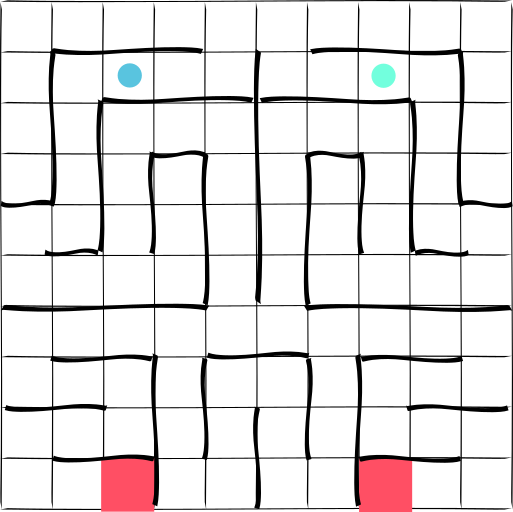
\includegraphics[width=0.5\textwidth,height=0.5\textheight]{../../pictures/drawings/maze.png}
\caption{maze.png}
\end{figure}

This reduces the state-action space by half!
\(\frac{1}{2}\mid S \mid \times \mid A \mid\). Note: just using state
abstraction it is not possible to achieve this reduction. Mirrored
states are not equivalent as the actions are inverted.

While other learners can still solve this problem. They miss out on
efficiency gains by abstracting first.

This intuition leads to our work in section ... (symetric abstractions).

\subsubsection{Temporal abstraction}

???


\hypertarget{related-work}{%
\subsubsection{Related work}\label{related-work}}

Other approaches to abstraction for RL focus on \ldots{}?

Near Optimal Behavior via Approximate State Abstraction \cite{Abel2017}
A Geometric Perspective on Optimal Representations for Reinforcement Learning \cite{Bellemare2019b}
successor representation

\hypertarget{discussion}{%
\subsection{Discussion}\label{discussion}}

But can we guarantee that these abstractions do not make it harder to
find the optimal policy? Is that even possible?

\begin{center}\rule{0.5\linewidth}{\linethickness}\end{center}

Want a general way (a function) to take an abstraction of an MDP
(defined by certain propreties) and return the difference between its
optimal policy and the true optimal policy. Want automated computational
complexity to solve this! Actually, we are not considering computational
complexity here only approximation error. For that can we just use
automatic differentiation!? Want a way to get bounds for all of these
combinations!

Requires the evaluation of expensive integrals?!?



***

The three steps of abstraction - relaxation (transform to a new domain)
- linearisation (and solve) -
